This section has the aim to aggregate all scores obtained in section 3 for each group, every value is computed as the average of heuristics' scores previously assigned and represents the overall evaluation about how navigation, contents and layout  is handled in "Visit Monterosa" website. Values are then approximeted by defect or by excess.

\subsubsection*{Navigation}
The navigation analysis is given by the five values corresponding to the 5 analyzed aspects: Interaction Consistency, Group Navigation, Structural Navigation, Semantic Navigation and Landmarks.\\
\textbf{Average: } ( 4 + 2.5 + 4.5 + 2 + 4) / 5 = 3.4  \emph{which can be approx to 3.5}\\
\begin{figure}[h!]
	\centering
	\begin{minipage}[b]{1\textwidth}
    		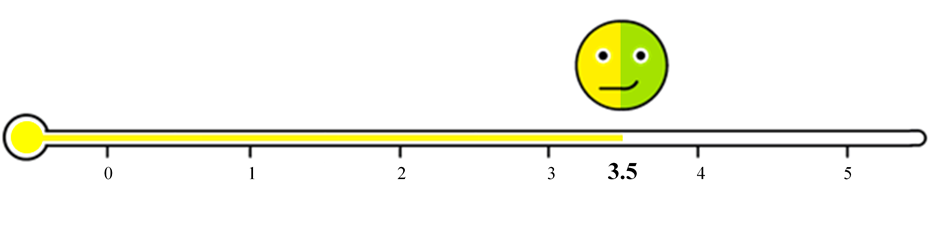
\includegraphics[width=1\textwidth]{./assets/layout-navigation-value.png}
	\end{minipage}
\end{figure}
\FloatBarrier

The mathematical average gives a 3.5 out of 5; this value underlines the fact that navigation is is pretty well handled, but with some issues that could be easily solved as reported in section 3.1.

\subsubsection*{Contents}
The overall evaluation about contents is given by the average of the 2 analyzed aspects.\\
\textbf{Average: } ( 3.5 + 4 ) / 2 = 3.75  \emph{which can be approx to 4}\\
\begin{figure}[h!]
	\centering
	\begin{minipage}[b]{1\textwidth}
    		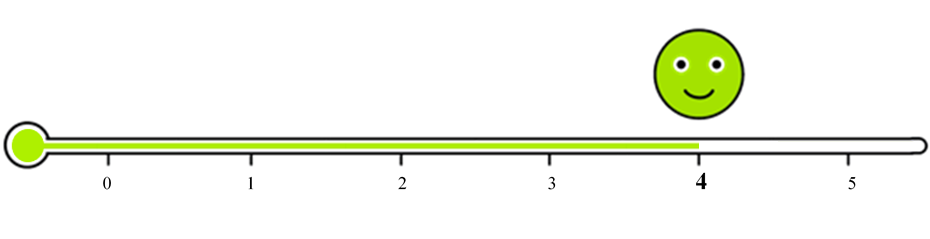
\includegraphics[width=1\textwidth]{./assets/contents-value.png}
	\end{minipage}
\end{figure}
\FloatBarrier

The mathematical average gives a 4 out of 5, a really high value. This evaluation is obtained because the website offers lots of information related to various topics and because they are quite well organized between pages. It could reach the maximum score by adding some little improvements as explained in section 3.2.

\subsubsection*{Layout}
For what concern the layout analysis, it has been done thanks to the evaluation of 4 foundamental aspects.\\
\textbf{Average: } ( 3 + 4 + 4 + 3 ) / 4 = 3.5 \\
\begin{figure}[h!]
	\centering
	\begin{minipage}[b]{1\textwidth}
    		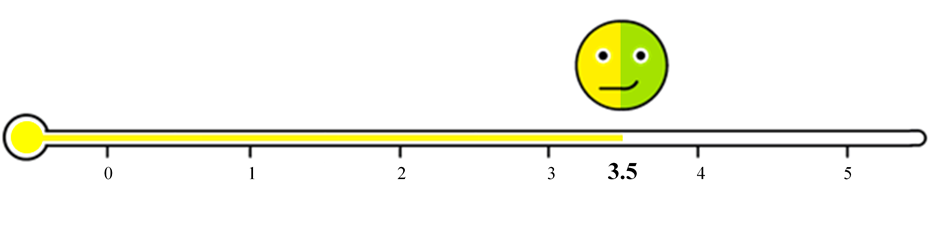
\includegraphics[width=1\textwidth]{./assets/layout-navigation-value.png}
	\end{minipage}
\end{figure}
\FloatBarrier

Also in this case the average gives a 3.5 out of 5; this value means that layout is pretty well done but could be improved more by adjusting some critical aspects such as Text Layout and the Concistency between pages.